\section{Setting up Problems and ODEs for a Single Particle}

A simple pendulum with a point mass is taken as an exemplar point particle problem. The second order equation of motion is written as a system of first order ODEs in julia.

\begin{equation}
    \ddot{\theta} + \frac{g}{l} \sin\left(\theta\right)
\end{equation}

where $g$ is the acceleration due to gravity, $l$ is the length of the string of the point-mass pendulum and $\theta(t)$ is the angle that the string makes with the normal axis.

\begin{minted}{julia}
function system!(du, u, p, t)
    # Unpack state vector
    ϕ_1, ϕ_2 = u
    l, g = p

    # Define time differentials
    dϕ_1 = ϕ_2
    dϕ_2 = -g/l * sin(ϕ_1)

    du[1] = dϕ_1
    du[2] = dϕ_2
    return nothing
end
\end{minted}

\begin{figure}[htbp]
    \centering
    \begin{subfigure}[b]{0.48\textwidth}
        \centering
        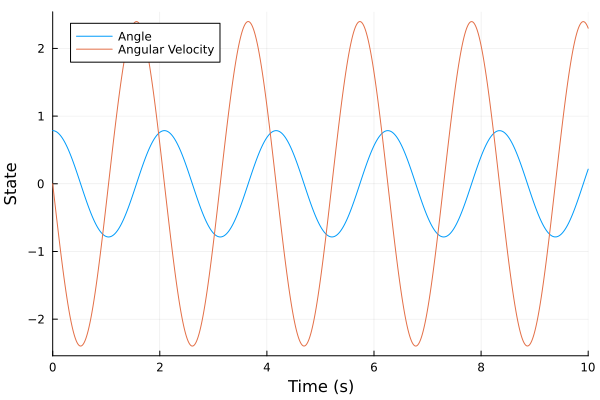
\includegraphics[width=\textwidth]{Problems/Problem1/figures/state_plot.png}
        \caption{Time-Dependent Solutions}
    \end{subfigure}
    \hfill
    \begin{subfigure}[b]{0.48\textwidth}
        \centering
        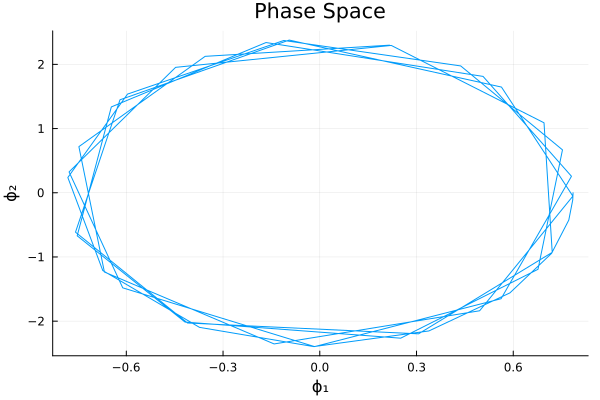
\includegraphics[width=\textwidth]{Problems/Problem1/figures/phase_space.png}
        \caption{Phase Space}
    \end{subfigure}
    \caption{Solution}
\end{figure}

The solution of the problem was animated.

\begin{minted}{julia}
animation = @animate for t in range(tspan[1], tspan[2], length = 200)
    θ = solution(t)[1]
    dθ = solution(t)[2] # We will not be using this result here

    x = l * sin(θ)
    y = -l * cos(θ)

    # Animate the string too!
    plot(
        [0, x],
        [0, y],
        lw = 3,
        color = :black,
        aspect_ratio =:equal,
        xlims=(-1.2l, 1.2l), ylims=(-1.2l, 0.2l)
    )

    # Animate the mass
    scatter!(
        [x], [y], color = :red, ms = 12
    )
end
\end{minted}